\documentclass[11pt]{article}

% ----------------------------------------------------------------------------
% ProPS-Twin -- Progress Report: Scenarios and Telemetry (Phase 3)
% Supervisor-facing. Every quantitative claim is taken from
% results/phase3/report.json or from commands recorded in Appendix A.
% ----------------------------------------------------------------------------

\usepackage[utf8]{inputenc}
\usepackage[T1]{fontenc}
\usepackage{lmodern}
\usepackage[a4paper,margin=1in]{geometry}
\usepackage{microtype}
\usepackage{xcolor}
\usepackage{graphicx}
\usepackage{booktabs}
\usepackage{array}
\usepackage{longtable}
\usepackage{tabularx}
\usepackage{ragged2e}
\setlength{\emergencystretch}{3em}
\usepackage{amsmath}
\usepackage{amssymb}
\usepackage{enumitem}
\usepackage{tikz}
\usetikzlibrary{arrows.meta,positioning,shapes.geometric,fit,backgrounds,calc}
\usepackage{pgfplots}
\pgfplotsset{compat=1.17}
\usepackage{fancyhdr}
\usepackage{abstract}
\usepackage[hidelinks]{hyperref}
\usepackage{titlesec}
\usepackage{caption}

\definecolor{navy}{HTML}{1f2a44}
\definecolor{accent}{HTML}{2c4fb0}
\definecolor{green}{HTML}{3a7d2c}
\definecolor{cyan}{HTML}{127a6e}
\definecolor{red}{HTML}{b03030}
\definecolor{amber}{HTML}{b07a10}
\definecolor{violet}{HTML}{6a3fa8}
\definecolor{gray}{HTML}{555555}
\definecolor{panel}{HTML}{f2f2f2}
\definecolor{panelline}{HTML}{cccccc}

\hypersetup{colorlinks=true,linkcolor=accent,urlcolor=accent,citecolor=accent}

\newcommand{\code}[1]{\texttt{\small #1}}
\newcommand{\file}[1]{\textcolor{navy}{\texttt{\small #1}}}
\newcommand{\done}{\textcolor{green}{\textbf{complete}}}
\newcommand{\stpartial}{\textcolor{amber}{\textbf{partial}}}
\newcommand{\todo}{\textcolor{red}{\textbf{not started}}}

\titleformat{\section}{\large\bfseries\color{navy}}{\thesection}{0.6em}{}
\titleformat{\subsection}{\normalsize\bfseries\color{accent}}{\thesubsection}{0.6em}{}

\pagestyle{fancy}
\fancyhf{}
\lhead{\small\textcolor{gray}{ProPS-Twin: Progress Report, Phase 3}}
\rhead{\small\textcolor{gray}{\thepage}}
\renewcommand{\headrulewidth}{0.3pt}

\captionsetup{font=small,labelfont=bf}

\begin{document}

% ---------------------------------------------------------------- title page
\begin{titlepage}
\centering
\vspace*{1.5cm}
{\color{navy}\rule{\linewidth}{1.4pt}}\\[10pt]
{\Huge\bfseries ProPS-Twin}\\[8pt]
{\LARGE An LLM-Guided Cybersecurity Digital Twin for\\ IT/OT Risk Propagation
and Defensive Policy Optimization}\\[10pt]
{\large Progress Report: Scenarios, Telemetry and the Experiment Ledger}\\[6pt]
{\color{navy}\rule{\linewidth}{1.4pt}}\\[1.4cm]

{\large\textbf{Scope of this report:}\\ proposal Phases 1--3, with the state of
Phases 4--6}\\[1.2cm]

\begin{tabular}{rl}
\textbf{Course} & CSE499A\\[2pt]
\textbf{Document type} & Formal progress report (supervisor-facing)\\[2pt]
\textbf{Repository} & \href{https://github.com/saifahmedarfi/twinward}{\file{github.com/saifahmedarfi/twinward}}, commit \code{83ff228}\\[2pt]
\textbf{Primary entry point} & \file{main.py} (\code{python main.py phase3})\\[2pt]
\textbf{Verification} & 86 automated tests pass (including PostgreSQL)\\[2pt]
\textbf{Experiments recorded} & 49 runs, 47{,}250 events, results of 2026-11-27\\[2pt]
\textbf{Reward model} & $R=w_dD+w_cC+w_aA+w_rQ-w_fF-w_lL$\\
\end{tabular}

\vfill
{\small This report separates what is implemented and measured from what is
planned. Numbers in the results sections are copied from the run record
\file{results/phase3/report.json}; nothing is estimated or rounded beyond the
precision shown. The environment is simulated and has no connection to any real
plant network or control system.}\\[6pt]
{\small\color{gray}Compiled 2026-11-27.}
\end{titlepage}

% ---------------------------------------------------------------- abstract
\begin{abstract}
\noindent
ProPS-Twin is a containerized cybersecurity digital twin of a representative
nuclear power plant IT department and its simulated boundary to operational
technology (OT). The proposal sets out six implementation phases, ending in a
Prompted Policy Search (ProPS) loop in which a large language model proposes
bounded defensive-policy parameters and a deterministic evaluator scores them.
This report covers the work completed up to the end of Phase 3, whose deliverable
in the proposal is ``a repeatable scenario runner, structured logs, and evaluation
records''. We describe the experiment lifecycle that now wraps every run
(configure, simulate, observe, evaluate, persist), the reset procedure that
returns the twin to a known baseline between candidate policies, and an
observability plane built from the tools named in the proposal: structured
JSON-lines logs, OpenTelemetry traces and trace-correlated log records,
Prometheus metrics, and a PostgreSQL experiment ledger, all deployed with Docker
Compose. In a 49-run campaign the seven scenarios reproduced exactly across
repeated runs, all seven passed a reset check that includes a negative control,
and every one of the 47{,}250 emitted events was found in the ledger and in the
OpenTelemetry Collector. Four fixed policy presets already expose the trade-offs
the optimizer will have to handle: a strict access profile raises the reward of
three scenarios from 0.60 to 0.85, a lockdown profile buys the same containment
at the cost of all legitimate inter-zone traffic, and a hair-trigger alert
threshold adds 24 to 27 false positives per run. The research core of the
project, the ProPS loop and its baselines, has not been started, and we say so
plainly. By phase count the project is about half complete.
\end{abstract}

\paragraph{Keywords.} cybersecurity digital twin; IT/OT security; cyber range;
Prompted Policy Search; OpenTelemetry; Prometheus; experiment reproducibility;
security telemetry.

\tableofcontents
\clearpage

% ================================================================ 1
\section{Introduction}
\label{sec:intro}
The proposal frames ProPS-Twin around one question: can prompt-guided policy
search improve defensive outcomes in an IT/OT environment while respecting hard
security and availability constraints? Answering it needs three things in
place before any language model is involved. The twin has to produce incidents
that are repeatable, so two candidate policies can be compared on the same
scenario and seed. Each run has to leave evidence that can be inspected and
re-scored later. And the environment has to return to the same starting state
between candidates, otherwise differences in reward could come from leftover
state rather than from the policy.

The earlier engineering report documented the simulated estate (five components
in four zones), the seven scenario definitions and the log-only evaluator. Those
pieces ran correctly but in isolation: the estate and reward configuration files
were never read, the reset procedure declared in each scenario was never
executed, the policy hook on every component was never called, and a run left
behind nothing more than an optional SQLite table. This report describes how
Phase 3 closed those gaps and what the resulting platform measured.

The report is organized as follows. Section~\ref{sec:progress} places the work
against the proposal's phases, objectives and research questions.
Sections~\ref{sec:arch}--\ref{sec:services} describe the architecture, the
experiment lifecycle, the scenario set, the reset path, the telemetry and
evidence plane, and the live service layer. Sections~\ref{sec:setup}
and~\ref{sec:results} give the experimental protocol and the results.
Section~\ref{sec:discussion} interprets them, Section~\ref{sec:validity} lists
threats to validity, and Section~\ref{sec:next} sets out the next phase.

% ================================================================ 2
\section{Progress against the proposal}
\label{sec:progress}

\subsection{Implementation phases}
Table~\ref{tab:phases} maps the six phases of the proposal (its Table~2) to their
current state. Phases 1--3 are complete. Phases 5 and 6 have some groundwork from
the containerized stack and the existing visualization, but neither is close to
its stated deliverable. Phase 4, which holds the research contribution, has not
been started.

\begin{table}[h]
\centering
\caption{Proposal implementation phases and their status on 2026-11-27.}
\label{tab:phases}
\small
\begin{tabular}{>{\RaggedRight\arraybackslash}p{0.6cm} >{\RaggedRight\arraybackslash}p{3.0cm} p{1.9cm} >{\RaggedRight\arraybackslash}p{8.2cm}}
\toprule
\textbf{\#} & \textbf{Focus} & \textbf{Status} & \textbf{Evidence}\\
\midrule
1 & Threat model and design & \done & Topology, zones, trust boundaries, scenarios, constraints and metrics in \file{docs/} and \file{configs/}\\
2 & Local digital twin & \done & Five simulated services; Docker images build and pass health checks\\
3 & Scenarios and telemetry & \done & This report: lifecycle, reset path, ledger, OpenTelemetry, Prometheus, Compose stack\\
4 & ProPS integration & \todo & \file{research/policy\_engine/}, \file{props\_optimizer/} and \file{baselines/} hold only READMEs\\
5 & LLM analyst and dashboard & \stpartial & Replay and live visualization exist (\file{viz/}); no LLM explanations\\
6 & Kubernetes deployment & \stpartial & Containerized stack with persistent volumes and a restart check; no Kubernetes manifests\\
\bottomrule
\end{tabular}
\end{table}

Counting complete phases gives three of six. Weighting by effort gives a less
flattering picture, because Phase 4 is the largest single piece of work left and
everything in RQ2 depends on it. A fair summary is that the platform is ready and
the experiment it was built for has not yet been run.

\subsection{Objectives}
\begin{table}[h]
\centering
\caption{Proposal objectives (Section 3) and their status.}
\label{tab:objectives}
\small
\begin{tabular}{>{\RaggedRight\arraybackslash}p{0.6cm} >{\RaggedRight\arraybackslash}p{7.4cm} p{1.9cm} >{\RaggedRight\arraybackslash}p{4.0cm}}
\toprule
& \textbf{Objective} & \textbf{Status} & \textbf{Where}\\
\midrule
O1 & Model a representative IT department, dependencies, access controls, monitoring and an OT-facing boundary & \done & \file{services/*/core.py}\\
O2 & Parameterized scenarios for excessive privileges, incomplete logging, weak segmentation, remote-access failure and outages & \done & Table~\ref{tab:scenarios}\\
O3 & Timestamped structured events and metrics for detection, containment, availability, false positives and recovery & \done & Sections~\ref{sec:telemetry}, \ref{sec:metrics}\\
O4 & ProPS loop: LLM proposes bounded parameters, simulator evaluates & \todo & Phase 4\\
O5 & Compare with baseline, expert policy, random search and a conventional optimizer & \todo & Phase 4\\
O6 & Package with Docker, deploy to Kubernetes, test log and experiment persistence & \stpartial & Section~\ref{sec:persist}\\
\bottomrule
\end{tabular}
\end{table}

\subsection{Research questions}
\begin{description}[leftmargin=1.2em,style=nextline]
\item[RQ1 (risk propagation)] Preliminary evidence is available. The policy-preset
matrix in Section~\ref{sec:levers} shows how a weak access profile lets violating
flows through on three scenarios and how tighter profiles change detection,
containment and availability. The experiments are not yet designed to isolate
propagation across zones.
\item[RQ2 (policy optimization)] Not yet addressable. It needs the ProPS loop and
the four baselines named in the proposal.
\item[RQ3 (deployment resilience)] One preliminary result: the experiment ledger
kept its full history across a database container restart, and an availability
probe correctly reported the simulated forwarder outage on the live service. A
systematic restart study belongs to Phase 6.
\end{description}

% ================================================================ 3
\section{System architecture after Phase 3}
\label{sec:arch}
The proposal describes ProPS-Twin as cooperating planes rather than a single
pipeline. Figure~\ref{fig:arch} shows how the implemented components now map onto
those planes. The policy-search plane is drawn dashed because it does not exist
yet; the runner exposes the call it will use.

\begin{figure}[h]
\centering
\resizebox{\linewidth}{!}{%
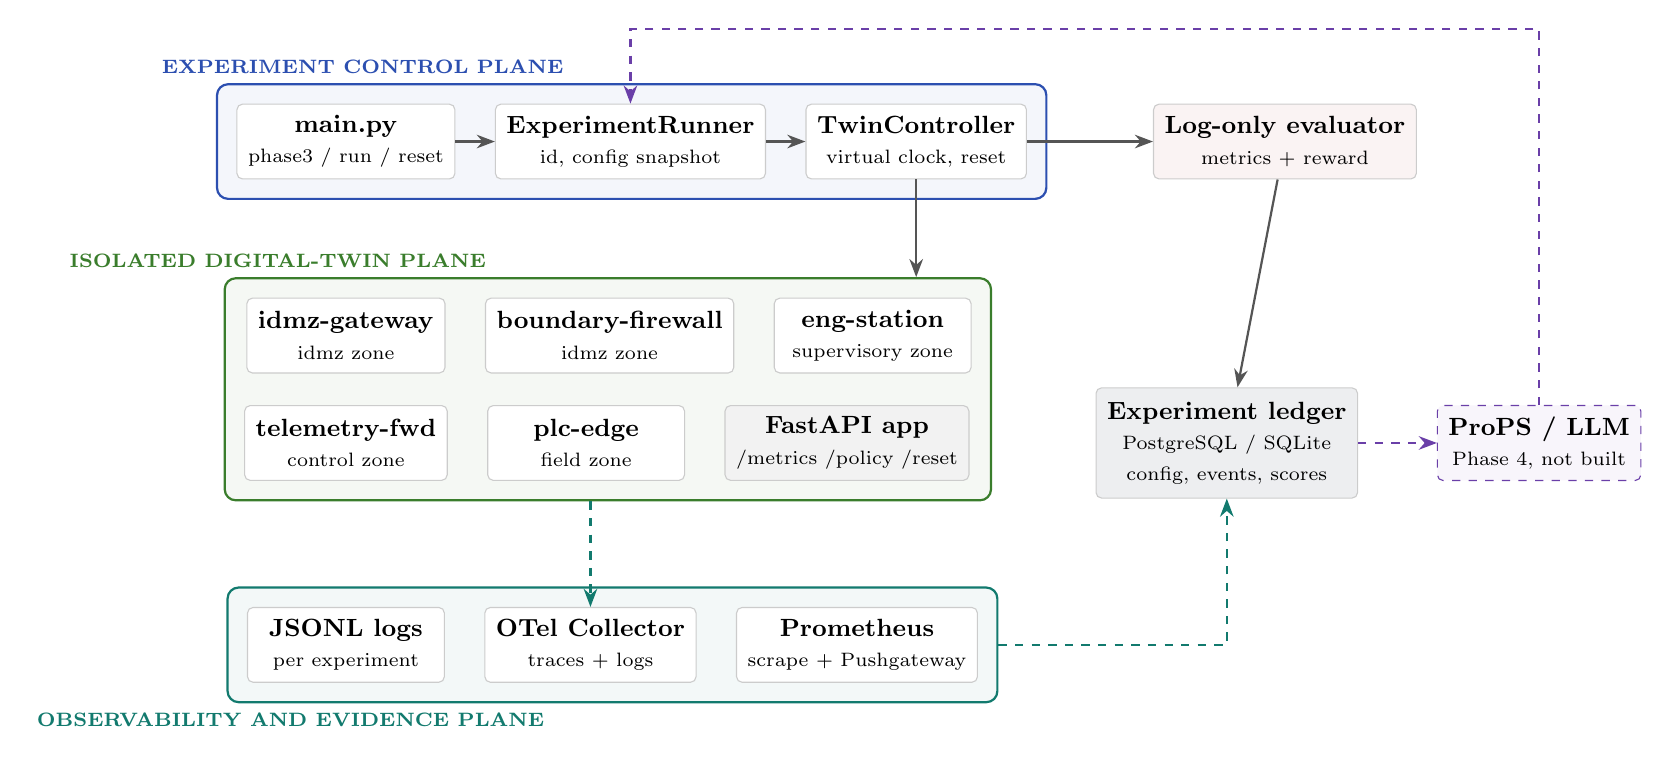
\begin{tikzpicture}[
  font=\small,
  box/.style={rectangle,rounded corners=2pt,draw=panelline,fill=white,
              align=center,inner sep=4pt,minimum height=0.95cm,minimum width=2.5cm},
  plane/.style={rectangle,rounded corners=4pt,draw=#1,thick,fill=#1!5,inner sep=7pt},
  arr/.style={-{Stealth[length=2.3mm]},thick,draw=gray},
  tel/.style={-{Stealth[length=2.3mm]},thick,draw=cyan,dashed},
  pol/.style={-{Stealth[length=2.3mm]},thick,draw=violet,dashed},
  ]
  % control plane
  \node[box] (main) {\textbf{main.py}\\\scriptsize phase3 / run / reset};
  \node[box,right=0.5cm of main] (runner) {\textbf{ExperimentRunner}\\\scriptsize id, config snapshot};
  \node[box,right=0.5cm of runner] (twin) {\textbf{TwinController}\\\scriptsize virtual clock, reset};

  % twin plane
  \node[box,below=1.5cm of main] (idmz) {\textbf{idmz-gateway}\\\scriptsize idmz zone};
  \node[box,right=0.5cm of idmz] (fw) {\textbf{boundary-firewall}\\\scriptsize idmz zone};
  \node[box,right=0.5cm of fw] (eng) {\textbf{eng-station}\\\scriptsize supervisory zone};
  \node[box,below=0.4cm of idmz] (fwd) {\textbf{telemetry-fwd}\\\scriptsize control zone};
  \node[box,right=0.5cm of fwd] (plc) {\textbf{plc-edge}\\\scriptsize field zone};
  \node[box,right=0.5cm of plc,fill=panel] (http) {\textbf{FastAPI app}\\\scriptsize /metrics /policy /reset};

  % observability plane
  \node[box,below=1.6cm of fwd] (jsonl) {\textbf{JSONL logs}\\\scriptsize per experiment};
  \node[box,right=0.5cm of jsonl] (otel) {\textbf{OTel Collector}\\\scriptsize traces + logs};
  \node[box,right=0.5cm of otel] (prom) {\textbf{Prometheus}\\\scriptsize scrape + Pushgateway};

  % evaluation, ledger, policy search
  \node[box,right=1.6cm of twin,fill=red!6] (eval) {\textbf{Log-only evaluator}\\\scriptsize metrics + reward};
  \node[box,right=1.6cm of http,fill=navy!8,minimum height=1.4cm] (ledger) {\textbf{Experiment ledger}\\\scriptsize PostgreSQL / SQLite\\\scriptsize config, events, scores};
  \node[box,right=1.0cm of ledger,draw=violet,dashed,fill=violet!5] (props) {\textbf{ProPS / LLM}\\\scriptsize Phase 4, not built};

  \begin{scope}[on background layer]
    \node[plane=accent,fit=(main)(runner)(twin),label={[font=\scriptsize\bfseries,text=accent]above left:EXPERIMENT CONTROL PLANE}] (cp) {};
    \node[plane=green,fit=(idmz)(eng)(fwd)(http),label={[font=\scriptsize\bfseries,text=green]above left:ISOLATED DIGITAL-TWIN PLANE}] (tp) {};
    \node[plane=cyan,fit=(jsonl)(otel)(prom),label={[font=\scriptsize\bfseries,text=cyan]below left:OBSERVABILITY AND EVIDENCE PLANE}] (op) {};
  \end{scope}

  \draw[arr] (main)--(runner);
  \draw[arr] (runner)--(twin);
  \draw[arr] (twin.south)--(twin.south|-tp.north);
  \draw[tel] (tp.south-|otel.north)--(otel.north);
  \draw[arr] (twin)--(eval);
  \draw[arr] (eval)--(ledger);
  \draw[tel] (op.east)-|(ledger.south);
  \draw[pol] (ledger)--(props);
  \draw[pol] (props.north)|-([yshift=0.95cm]runner.north)--(runner.north);
\end{tikzpicture}}
\caption{Plane-based architecture as implemented. Solid arrows are control and
data flow; cyan dashed arrows are telemetry; violet dashed arrows are the planned
policy feedback path. The LLM will have no direct path into the twin plane: its
only output will be a candidate policy passed to \code{ExperimentRunner.run}.}
\label{fig:arch}
\end{figure}

Two properties from the previous design are kept on purpose. First, the
simulation cores remain standard-library Python and know nothing about
telemetry: every exporter is attached to the event sink as a hook. Second, ground
truth never enters the event stream. Trace and span identifiers are written to
the ledger and to the log files, never into the event records the detector reads,
so adding observability did not give the detector a way to cheat.

% ================================================================ 4
\section{The experiment lifecycle}
\label{sec:lifecycle}
Every experiment, whether started by hand or, later, by the optimizer, goes
through the same five steps. These are the first four steps of the proposal's
Figure~2 plus an explicit persistence step.

\begin{figure}[h]
\centering
\resizebox{0.95\linewidth}{!}{%
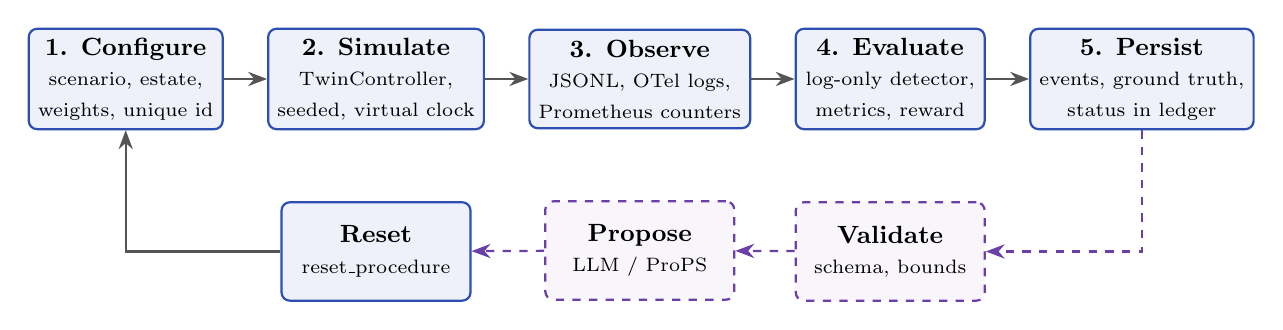
\begin{tikzpicture}[
  font=\small,
  st/.style={rectangle,rounded corners=3pt,draw=accent,fill=accent!8,thick,
             align=center,minimum width=2.4cm,minimum height=1.25cm},
  fut/.style={st,draw=violet,fill=violet!5,dashed},
  arr/.style={-{Stealth[length=2.4mm]},thick,draw=gray},
  ]
  \node[st] (c) {\textbf{1. Configure}\\\scriptsize scenario, estate,\\\scriptsize weights, unique id};
  \node[st,right=0.55cm of c] (s) {\textbf{2. Simulate}\\\scriptsize TwinController,\\\scriptsize seeded, virtual clock};
  \node[st,right=0.55cm of s] (o) {\textbf{3. Observe}\\\scriptsize JSONL, OTel logs,\\\scriptsize Prometheus counters};
  \node[st,right=0.55cm of o] (e) {\textbf{4. Evaluate}\\\scriptsize log-only detector,\\\scriptsize metrics, reward};
  \node[st,right=0.55cm of e] (p) {\textbf{5. Persist}\\\scriptsize events, ground truth,\\\scriptsize status in ledger};
  \node[fut,below=0.9cm of e] (v) {\textbf{Validate}\\\scriptsize schema, bounds};
  \node[fut,below=0.9cm of o] (pr) {\textbf{Propose}\\\scriptsize LLM / ProPS};
  \node[st,below=0.9cm of s,minimum width=2.4cm] (r) {\textbf{Reset}\\\scriptsize reset\_procedure};
  \draw[arr] (c)--(s); \draw[arr] (s)--(o); \draw[arr] (o)--(e); \draw[arr] (e)--(p);
  \draw[arr,draw=violet,dashed] (p.south)|-(v.east);
  \draw[arr,draw=violet,dashed] (v)--(pr);
  \draw[arr,draw=violet,dashed] (pr)--(r);
  \draw[arr] (r.west)-|(c.south);
\end{tikzpicture}}
\caption{Experiment lifecycle. Solid boxes are implemented. The dashed boxes are
Phase 4; until then the next candidate is a preset or a command-line override.}
\label{fig:lifecycle}
\end{figure}

\paragraph{Configure.} The runner loads the scenario, the estate configuration
(\file{estate-config.yaml}) and the reward weights (\file{reward.yaml}), both
under \file{configs/}. Before Phase 3 neither file was read.
It then asks the ledger for the next free run counter for the
\emph{(scenario, seed)} pair, which gives every experiment a unique identifier of
the form \code{exp-SC-04-1004-0007}. Repeated runs therefore never overwrite
earlier evidence. A snapshot of the scenario, estate and weights is stored with
the record.

\paragraph{Policy resolution.} The policy that is actually in force is built in
three layers, each overriding the one before:
\begin{equation}
\pi_{\text{eff}} \;=\; \pi_{\text{estate}} \;\oplus\; \pi_{\text{scenario}} \;\oplus\; \pi_{\text{candidate}},
\end{equation}
where $\pi_{\text{estate}}$ is the baseline declared in the estate file,
$\pi_{\text{scenario}}$ comes from the scenario's \code{initial\_conditions}, and
$\pi_{\text{candidate}}$ is a preset or an override. Components boot with the
first two layers. The candidate is applied on top through each component's
\code{apply\_policy()} method, which existed before Phase 3 but had no caller.
Keeping the candidate separate is what lets the reset step restore the baseline
without rebuilding the configuration. Four levers are exposed: alert threshold
(1--5), IDMZ access profile (standard, strict, lockdown), boundary rate limit and
recovery timeout.

\paragraph{Simulate and observe.} The \code{TwinController} steps a virtual clock
over the evaluation window and applies the scheduled mode changes. Each emitted
event passes through three observers: the per-experiment JSONL log, an
OpenTelemetry log record and a Prometheus counter. Each mode change also becomes a
span event on the simulate span, with its simulated time.

\paragraph{Evaluate and persist.} The evaluator is unchanged from the earlier
report apart from receiving the effective alert threshold, recovery budget and
weights. The runner adds the containment and resilience counts listed in
Section~\ref{sec:metrics}, writes events and ground truth to the ledger, counts
how many events the ledger now holds for the experiment, and marks the record
\code{completed}. An exception marks it \code{failed} with the error text, so a
crash is visible in the ledger rather than silently missing.

% ================================================================ 5
\section{Scenario design}
\label{sec:scenarios}
The proposal's Table~1 lists five controlled conditions. Table~\ref{tab:scenarios}
shows which scenario realizes each one. Segmentation misconfiguration is covered
three times because the boundary is where most of the policy levers act.

\begin{table}[h]
\centering
\caption{Proposal conditions and the scenarios that implement them.}
\label{tab:scenarios}
\small
\begin{tabular}{p{1.1cm} >{\RaggedRight\arraybackslash}p{3.7cm} >{\RaggedRight\arraybackslash}p{5.0cm} >{\RaggedRight\arraybackslash}p{3.6cm}}
\toprule
\textbf{ID} & \textbf{Proposal condition} & \textbf{Injected fault (window, component)} & \textbf{Detection}\\
\midrule
SC-01 & Segmentation misconfiguration & Non-whitelisted inter-zone protocol, $t\in[30,50]$, idmz-gateway & presence, drop-rate threshold\\
SC-02 & Segmentation / boundary & Broadcast packet storm, $[40,55]$, boundary-firewall & presence, drop-rate threshold\\
SC-03 & Excessive privileges & Privileged command by an operator identity, $[50,51]$, eng-station & presence, violation state\\
SC-04 & Segmentation misconfiguration & Jump-host crossing to a control destination, $[35,45]$, idmz-gateway & presence, violation state\\
SC-05 & Incomplete logging & Required audit record omitted, $[40,70]$, eng-station & absence, 5\,s timeout\\
SC-06 & Remote-access policy failure & Unauthenticated remote access, $[45,53]$, idmz-gateway & presence, violation state\\
SC-07 & Monitoring/service outage & Data-diode heartbeat pause, $[40,60]$, telemetry-forwarder & absence, 5\,s timeout, recovery\\
\bottomrule
\end{tabular}
\end{table}

\paragraph{Schema validation.} Scenarios are now validated by a Pydantic v2 model
(Step 3.1 of the handbook). It rejects an unknown action or target component, an
inverted ground-truth window, a window that ends after the evaluation window, an
unknown reset step, and a probe section with a zero interval. Six malformed
variants are covered by tests. When Pydantic is not installed the earlier plain
validator runs instead, so the standard-library path still works.

\paragraph{Availability probes.} Only SC-07 used to probe availability, which meant
the availability term $A$ was fixed at its neutral value of 1.0 for every
boundary scenario and could not penalize an over-restrictive policy. SC-04 and
SC-06 now probe the IDMZ gateway every 10\,s. Under the standard profile all 12
probes succeed, so baseline rewards did not move. SC-01 was left untouched to keep
its event stream identical to earlier runs.

% ================================================================ 6
\section{The reset path}
\label{sec:reset}
Each scenario declares a \code{reset\_procedure}; until this phase nothing executed
it and \code{make reset} printed a placeholder. \code{TwinController.reset()} now
runs the declared steps in order:
\begin{enumerate}[leftmargin=1.6em,itemsep=1pt]
\item \code{restore\_modes}: every component returns to mode \code{normal}, and any
pending buffer drain on the forwarder is cleared;
\item \code{restore\_policy\_baseline}: the baseline value of every lever is written
back through \code{apply\_policy()} and the active candidate is cleared;
\item \code{flush\_state}: every component is rebuilt from the global seed, which
resets the random streams, counters and uptime, and the event sink is emptied;
\item \code{new\_experiment\_id}: the run counter advances.
\end{enumerate}
A run on a twin that has already run (a ``dirty'' twin) resets automatically
first. One detail needed care: if a caller sets the next candidate and then runs,
the automatic reset must not wipe that candidate. The controller saves the
pending policy across the reset and reapplies it, and a test covers this case.

\paragraph{How the reset is checked.} Showing that a re-run after reset matches the
first run is not enough on its own, because that would also hold if the
simulation ignored its state altogether. The check therefore has a negative
control: the same twin is run a third time with the reset bypassed. A working
reset should make the second run identical to the first, and skipping it should
make the third run differ. Payloads are compared field by field (timestamp,
component, event type, severity, state and details), excluding the identifiers
that are supposed to change.

% ================================================================ 7
\section{Telemetry and evidence}
\label{sec:telemetry}
The proposal's tooling section names structured application logs,
OpenTelemetry-compatible instrumentation, Prometheus-style metrics and PostgreSQL
or an equivalent store. We gave each tool one job, so that no two of them hold
the authoritative copy of the same fact:
\begin{itemize}[leftmargin=1.4em,itemsep=1pt]
\item the \textbf{ledger} is the record of what happened and what it scored;
\item \textbf{OpenTelemetry} carries correlated evidence about how a run unfolded;
\item \textbf{Prometheus} holds numbers meant for dashboards and alerting;
\item \textbf{JSONL files} are the raw, greppable log of each experiment.
\end{itemize}

\subsection{Structured logs}
Every experiment writes \file{results/logs/<experiment\_id>.jsonl}. Each line is the
event exactly as emitted plus the run's \code{trace\_id} and \code{span\_id}. The
live services also print every event as one JSON line on standard output, which
is what a container runtime or a log shipper such as a Wazuh agent would collect.

\subsection{OpenTelemetry traces and logs}
Each experiment is one trace. Table~\ref{tab:spans} lists its spans. One OTel log
record is emitted per estate event inside the simulate span, so every record
carries the trace and span identifiers without any extra bookkeeping. Records are
exported over OTLP/HTTP to the collector when \code{OTEL\_EXPORTER\_OTLP\_ENDPOINT}
is set, and always to local JSONL files, so evidence exists even with no collector
running. The collector batches traces and logs and writes them to
\file{results/collector/}.

\begin{table}[h]
\centering
\caption{Span structure of one experiment trace.}
\label{tab:spans}
\small
\begin{tabular}{>{\RaggedRight\arraybackslash}p{4.0cm} >{\RaggedRight\arraybackslash}p{9.6cm}}
\toprule
\textbf{Span} & \textbf{Attributes and events}\\
\midrule
\code{experiment.run} & experiment id, scenario, seed, policy version, policy hash and parameters, code version; final status, reward and event count\\
\code{experiment.configure} & ledger backend\\
\code{experiment.simulate} & window end; one \code{scenario.action} span event per mode change (simulated $t$, target, mode, inject or restore); parent of all event log records\\
\code{experiment.evaluate} & \code{evaluation.result} span event with $R$ and all six components\\
\code{experiment.persist} & wraps the ledger write\\
\bottomrule
\end{tabular}
\end{table}

\subsection{Prometheus metrics}
Two sets of metrics are exported (Table~\ref{tab:prom}). The services expose
\code{/metrics} and Prometheus scrapes them every 5\,s. Batch experiments are
short-lived, so the runner pushes its registry to a Pushgateway at the end of a
campaign, the standard Prometheus pattern for batch jobs, and also writes a
textfile copy to \file{results/metrics/props\_twin.prom}. The collector's own
metrics are scraped as well, which gives an independent count of accepted spans
and log records.

\begin{table}[h]
\centering
\caption{Prometheus metric families.}
\label{tab:prom}
\footnotesize
\begin{tabular}{>{\RaggedRight\arraybackslash}p{6.5cm} >{\RaggedRight\arraybackslash}p{7.1cm}}
\toprule
\textbf{Metric} & \textbf{Meaning (labels)}\\
\midrule
\multicolumn{2}{l}{\emph{Experiment runner (Pushgateway / textfile)}}\\
\code{props\_events\_total} & events emitted (scenario, component, event type, severity, state)\\
\code{props\_runs\_total} & runs by final status (scenario, status)\\
\code{props\_resets\_total} & executed reset procedures (scenario)\\
\code{props\_reward}, \code{props\_reward\_component} & $R$ and D, C, A, Q, F, L of the latest run (scenario, policy version)\\
\code{props\_detection\_count} & TP, FP, FN, G and alerts of the latest run\\
\code{props\_detection\_delay\_seconds} & mean detection delay\\
\code{props\_log\_retention\_ratio} & persisted / emitted event records\\
\code{props\_prohibited\_flows} & violating flows not contained\\
\code{props\_run\_duration\_seconds} & wall-clock run duration (histogram)\\
\midrule
\multicolumn{2}{l}{\emph{Live services (scraped)}}\\
\code{props\_service\_events\_total} & events emitted by the live service\\
\code{props\_service\_ticks\_total}, \code{props\_service\_healthy} & tick count and health (1 or 0)\\
\code{props\_service\_mode\_info} & current simulated mode\\
\code{props\_service\_probe\_latency\_ms} & availability probe latency (histogram, ok label)\\
\code{props\_service\_policy\_applied\_total} & policy updates applied\\
\bottomrule
\end{tabular}
\end{table}

\subsection{The experiment ledger}
The proposal (Section 6.1) asks each experiment to record ``a unique ID,
timestamp, scenario seed, initial configuration, policy parameters, generated
event identifiers, metrics, reward, and final status''. Table~\ref{tab:ledger}
shows where each item is stored. The same schema runs on PostgreSQL (selected by
\code{PROPS\_DB\_URL}) or SQLite (the default), behind one small adapter, so a
laptop run and a stack run produce comparable records. Events are stored as rows
with their full details, which means a run can be re-scored from the ledger
without simulating it again.

\begin{table}[h]
\centering
\caption{Ledger tables and how they meet the proposal's record requirements.}
\label{tab:ledger}
\small
\begin{tabular}{>{\RaggedRight\arraybackslash}p{2.4cm} >{\RaggedRight\arraybackslash}p{11.2cm}}
\toprule
\textbf{Table} & \textbf{Contents}\\
\midrule
\code{experiments} & id, scenario, seed, run counter, status, created and finished timestamps, duration, policy version and parameters, configuration snapshot, reward, components, metrics, counts, events emitted and persisted, SHA-256 over the ordered event ids, trace id, code version, error\\
\code{events} & one row per event: id, timestamp, component, type, severity, state, zone, policy version, details\\
\code{ground\_truth} & labelled windows per experiment\\
\code{resets} & scenario, from and to experiment, steps executed, whether all components ended normal\\
\bottomrule
\end{tabular}
\end{table}

\paragraph{Correlation keys.} Three identifiers tie the stores together.
\code{experiment\_id} appears everywhere; \code{event\_id} links a ledger row, a
JSONL line and an OTel log record; \code{trace\_id} links a ledger record to its
spans and log records in the collector. Given any one of them, the rest of the
evidence for that run can be found.

% ================================================================ 8
\section{Live service layer and deployment}
\label{sec:services}
The five FastAPI wrappers were near-identical copies with a frozen clock (every
tick was $t=0$), no configuration and copied docstrings. They are now built by
one factory, \file{services/common/app.py}, and each \file{main.py} is a few lines
long. Table~\ref{tab:endpoints} lists the endpoints. Each service reads the estate
file mounted read-only, emits telemetry once per second, and exports events to
Prometheus and the collector.

\begin{table}[h]
\centering
\caption{HTTP surface of every estate service.}
\label{tab:endpoints}
\small
\begin{tabular}{>{\RaggedRight\arraybackslash}p{4.2cm} >{\RaggedRight\arraybackslash}p{9.4cm}}
\toprule
\textbf{Endpoint} & \textbf{Purpose}\\
\midrule
\code{GET /healthz}, \code{GET /state} & liveness; mode, health, tick count, zone, seed\\
\code{POST /control/mode} & inject or clear a simulated fault\\
\code{POST /policy} & apply allow-listed levers through \code{apply\_policy()}; empty body rejected (422)\\
\code{POST /tick?n=} & advance $n$ ticks, bounded to $[1, 10000]$\\
\code{GET /probe} & legitimate availability probe; 404 for components without one\\
\code{POST /reset} & fresh seeded state, baseline policy, cleared buffers\\
\code{GET /events?limit=} & most recent events (ring buffer of 500)\\
\code{GET /metrics} & Prometheus exposition\\
\code{POST /request} & IDMZ gateway only: broker an inter-zone request\\
\bottomrule
\end{tabular}
\end{table}

\begin{table}[h]
\centering
\caption{Docker Compose stack. All ports bind to 127.0.0.1 only.}
\label{tab:stack}
\small
\begin{tabular}{>{\RaggedRight\arraybackslash}p{2.7cm} >{\RaggedRight\arraybackslash}p{6.6cm} >{\RaggedRight\arraybackslash}p{4.3cm}}
\toprule
\textbf{Service} & \textbf{Image} & \textbf{Port / storage}\\
\midrule
5 estate services & \code{props-twin/*:dev} (python:3.12-slim) & 8001--8005; health-checked\\
OTel Collector & {\scriptsize\texttt{otel/opentelemetry-collector-contrib:0.111.0}} & OTLP 4317/4318; file export to \file{results/collector/}\\
Prometheus & \code{prom/prometheus:v2.55.1} & 9090; named volume, 7-day retention\\
Pushgateway & \code{prom/pushgateway:v1.10.0} & 9091\\
PostgreSQL ledger & \code{postgres:16-alpine} & 55432; named volume\\
\bottomrule
\end{tabular}
\end{table}

% ================================================================ 9
\section{Evaluation metrics}
\label{sec:metrics}
The reward is unchanged:
\begin{equation}
R(\pi) = w_dD + w_cC + w_aA + w_rQ - w_fF - w_lL,
\end{equation}
with weights now read from \file{reward.yaml}: $w_d=0.30$, $w_c=0.25$,
$w_a=0.20$, $w_r=0.10$, $w_f=0.10$, $w_l=0.05$. The maximum is 0.85, reached when
the four positive terms are 1 and both penalties are 0. A test confirms the file
is live: setting $w_c=0$ moves the SC-04 reward to exactly $0.30+0.20+0.10=0.60$.

The proposal's Table~3 lists metrics that the reward alone does not report. Each
ledger record now also carries the following:
\begin{itemize}[leftmargin=1.4em,itemsep=1pt]
\item \textbf{blocked and prohibited flow counts}: violating or anomalous events
that were, or were not, contained before effect (containment dimension);
\item \textbf{recovery time} in seconds from the end of a fault until the monitored
signal is healthy again (resilience dimension);
\item \textbf{retained event records} and \textbf{log retention}: events found in the
ledger after persistence, divided by events emitted, plus the JSONL line count;
\item \textbf{precision}, \textbf{false-positive rate} and \textbf{mean detection delay},
which were computed before but not stored.
\end{itemize}

% ================================================================ 10
\section{Experimental setup}
\label{sec:setup}
\paragraph{Environment.} Ubuntu (Linux 7.0), Python 3.14.4 on the host, Python 3.12
in the service images, Docker 29.7.2. Host libraries: OpenTelemetry SDK 1.45.2,
\code{prometheus\_client} 0.26.0, psycopg 3.3.9, Pydantic 2.14.3. The full stack
of Table~\ref{tab:stack} was running, with the runner exporting to PostgreSQL,
the collector and the Pushgateway.

\paragraph{Protocol.} One invocation of \code{python main.py phase3} ran three
blocks against the same ledger:
\begin{enumerate}[leftmargin=1.6em,itemsep=1pt]
\item the baseline suite, SC-01 to SC-07, repeated three times (21 experiments);
\item one reset cycle per scenario: run, reset, re-run, plus the no-reset control
(7 recorded resets);
\item a policy-preset matrix of seven scenarios by four presets (28 experiments).
\end{enumerate}
The four presets live in \file{configs/policies/}. \emph{baseline-v1} is the fixed
initial configuration. \emph{strict-v1} uses the strict access profile and a rate
limit of 40. \emph{lockdown-v1} uses the lockdown profile and a rate limit of 20.
\emph{sensitive-v1} lowers the alert threshold to 1 and the recovery budget to
30\,s. These presets are hand-chosen points used to check that each lever works.
They are not the expert-authored baseline the proposal calls for, and nothing here
is an optimization result.

\paragraph{Provenance.} The campaign ran at 2026-11-27 08:08 UTC on the working tree
that was committed immediately afterwards as \code{83ff228}. The ledger's
\code{code\_version} field shows the parent commit, \code{7adbd37}, because the
field records \code{HEAD} and does not yet flag uncommitted changes
(Section~\ref{sec:validity}). The campaign took 13.65\,s of wall time.

% ================================================================ 11
\section{Results}
\label{sec:results}

\subsection{Baseline suite}
Table~\ref{tab:baseline} gives the baseline results. They match the previous
report's figures exactly, which confirms that wiring in the configuration files,
the policy path and the new probes changed no baseline behavior.

\begin{table}[h]
\centering
\caption{Baseline policy, one representative run per scenario (all three repeats identical).}
\label{tab:baseline}
\small
\setlength{\tabcolsep}{4pt}
\begin{tabular}{l r r c c c c c c c c c}
\toprule
\textbf{ID} & \textbf{Events} & \textbf{$R$} & \textbf{D} & \textbf{C} & \textbf{A} & \textbf{Q} & \textbf{F} & \textbf{L} & \textbf{TP/FP/FN} & \textbf{Blk/Proh} & \textbf{Probes}\\
\midrule
SC-01 & 968 & 0.8500 & 1.00 & 1.00 & 1.00 & 1.00 & 0.000 & 0.000 & 20/0/0 & 0/0 & --\\
SC-02 & 983 & 0.8500 & 1.00 & 1.00 & 1.00 & 1.00 & 0.000 & 0.000 & 15/0/0 & 15/0 & --\\
SC-03 & 967 & 0.6000 & 1.00 & 0.00 & 1.00 & 1.00 & 0.000 & 0.000 & 1/0/0 & 0/1 & --\\
SC-04 & 980 & 0.6000 & 1.00 & 0.00 & 1.00 & 1.00 & 0.000 & 0.000 & 10/0/0 & 0/10 & 12/12\\
SC-05 & 938 & 0.8479 & 1.00 & 1.00 & 1.00 & 1.00 & 0.000 & 0.042 & 1/0/0 & 0/0 & --\\
SC-06 & 980 & 0.6000 & 1.00 & 0.00 & 1.00 & 1.00 & 0.000 & 0.000 & 8/0/0 & 0/8 & 12/12\\
SC-07 & 934 & 0.7879 & 1.00 & 1.00 & 0.75 & 0.90 & 0.000 & 0.042 & 1/0/0 & 0/0 & 9/12\\
\bottomrule
\end{tabular}
\end{table}

Three scenarios (SC-03, SC-04, SC-06) score 0.60 because the incident is detected
but not contained: one privileged command, ten jump-host crossings and eight
unauthenticated access attempts got through under the standard profile. The two
absence scenarios lose 0.042 on $L$ because a gap is only declared after the 5\,s
timeout, which gives a measured detection delay of 5.0\,s. SC-07 is the only
scenario with a measurable recovery time: the forwarder drains its buffer for 6\,s
after the pause ends, so $Q = 1 - 6/60 = 0.90$, and three of its twelve probes fall
inside the outage, so $A=0.75$.

\subsection{Reproducibility}
Each scenario was run three times under the baseline policy with a fresh
experiment identifier each time. All 21 runs reproduced their scenario's reward
exactly (Table~\ref{tab:baseline}), and their event payloads are identical up to
the identifiers. The full suite of seven runs takes 0.22--0.33\,s per experiment
including all exporters.

\subsection{Reset path}
All seven scenarios passed (Table~\ref{tab:reset}). In every case the four steps
ran, all components ended in mode \code{normal}, the re-run reproduced the first
run, and the control run without a reset did \emph{not}. The control matters: it
shows the identical second run is produced by the reset and not by a simulation
that ignores its own state.

\begin{table}[h]
\centering
\caption{Reset cycle per scenario.}
\label{tab:reset}
\small
\begin{tabular}{l l c c c c}
\toprule
\textbf{ID} & \textbf{First $\to$ second run} & \textbf{All normal} & \textbf{Same after reset} & \textbf{Same, no reset} & \textbf{New id}\\
\midrule
SC-01 & \code{...-1001-0004} $\to$ \code{0005} & yes & yes & no & yes\\
SC-02 & \code{...-1002-0004} $\to$ \code{0005} & yes & yes & no & yes\\
SC-03 & \code{...-1003-0004} $\to$ \code{0005} & yes & yes & no & yes\\
SC-04 & \code{...-1004-0004} $\to$ \code{0005} & yes & yes & no & yes\\
SC-05 & \code{...-1005-0004} $\to$ \code{0005} & yes & yes & no & yes\\
SC-06 & \code{...-1006-0004} $\to$ \code{0005} & yes & yes & no & yes\\
SC-07 & \code{...-1007-0004} $\to$ \code{0005} & yes & yes & no & yes\\
\bottomrule
\end{tabular}
\end{table}

\subsection{Policy-preset matrix}
\label{sec:levers}
Figure~\ref{fig:presets} plots the reward of each scenario under the four presets,
and Table~\ref{tab:presets} gives the components that changed.

\begin{figure}[h]
\centering
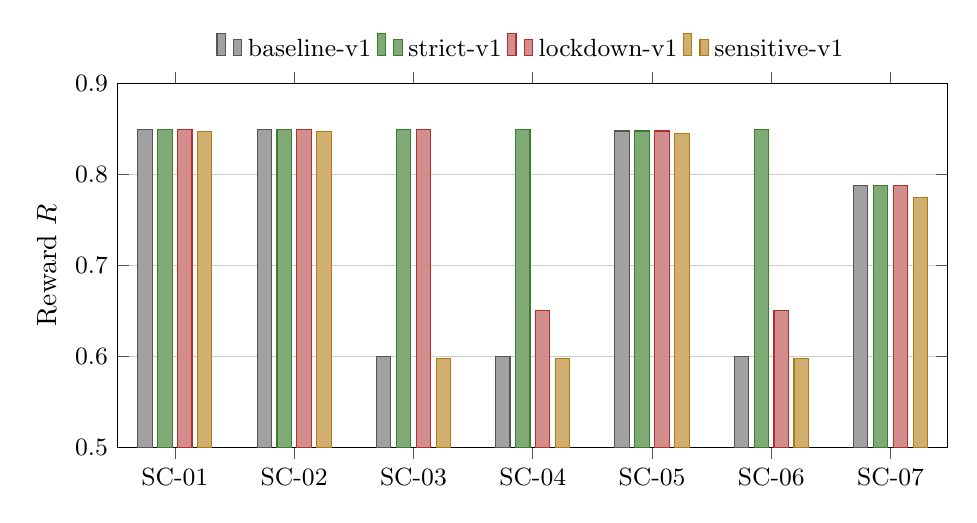
\begin{tikzpicture}
\begin{axis}[
  ybar, bar width=5.2pt, width=\linewidth, height=6.2cm,
  ymin=0.5, ymax=0.9, ylabel={Reward $R$},
  symbolic x coords={SC-01,SC-02,SC-03,SC-04,SC-05,SC-06,SC-07},
  xtick=data, enlarge x limits=0.08,
  legend style={at={(0.5,1.03)},anchor=south,legend columns=4,font=\small,draw=none},
  ymajorgrids, grid style={draw=panelline},
  tick label style={font=\small},
  ]
\addplot[fill=gray!55,draw=gray] coordinates {(SC-01,0.85) (SC-02,0.85) (SC-03,0.60) (SC-04,0.60) (SC-05,0.8479) (SC-06,0.60) (SC-07,0.7879)};
\addplot[fill=green!65,draw=green] coordinates {(SC-01,0.85) (SC-02,0.85) (SC-03,0.85) (SC-04,0.85) (SC-05,0.8479) (SC-06,0.85) (SC-07,0.7879)};
\addplot[fill=red!55,draw=red] coordinates {(SC-01,0.85) (SC-02,0.85) (SC-03,0.85) (SC-04,0.65) (SC-05,0.8479) (SC-06,0.65) (SC-07,0.7879)};
\addplot[fill=amber!60,draw=amber] coordinates {(SC-01,0.8475) (SC-02,0.8473) (SC-03,0.5972) (SC-04,0.5974) (SC-05,0.8447) (SC-06,0.5973) (SC-07,0.7746)};
\legend{baseline-v1, strict-v1, lockdown-v1, sensitive-v1}
\end{axis}
\end{tikzpicture}
\caption{Reward per scenario under four fixed policy presets (28 experiments).
The $y$ axis starts at 0.5 to make the small false-positive penalties visible.}
\label{fig:presets}
\end{figure}

\begin{table}[h]
\centering
\caption{Preset effects. Only rows where a component moved from baseline are shown; all other cells equal Table~\ref{tab:baseline}.}
\label{tab:presets}
\small
\begin{tabular}{l l r c c c c r r}
\toprule
\textbf{ID} & \textbf{Preset} & \textbf{$R$} & \textbf{C} & \textbf{A} & \textbf{Q} & \textbf{F} & \textbf{FP} & \textbf{Prohibited}\\
\midrule
SC-03 & strict-v1   & 0.8500 & 1.00 & 1.00 & 1.00 & 0.000 & 0  & 0\\
SC-03 & lockdown-v1 & 0.8500 & 1.00 & 1.00 & 1.00 & 0.000 & 0  & 0\\
SC-04 & strict-v1   & 0.8500 & 1.00 & 1.00 & 1.00 & 0.000 & 0  & 0\\
SC-04 & lockdown-v1 & 0.6500 & 1.00 & \textbf{0.00} & 1.00 & 0.000 & 0  & 0\\
SC-06 & strict-v1   & 0.8500 & 1.00 & 1.00 & 1.00 & 0.000 & 0  & 0\\
SC-06 & lockdown-v1 & 0.6500 & 1.00 & \textbf{0.00} & 1.00 & 0.000 & 0  & 0\\
\midrule
SC-01 & sensitive-v1 & 0.8475 & 1.00 & 1.00 & 1.00 & 0.025 & 24 & 0\\
SC-02 & sensitive-v1 & 0.8473 & 1.00 & 1.00 & 1.00 & 0.027 & 26 & 0\\
SC-03 & sensitive-v1 & 0.5972 & 0.00 & 1.00 & 1.00 & 0.028 & 27 & 1\\
SC-04 & sensitive-v1 & 0.5974 & 0.00 & 1.00 & 1.00 & 0.026 & 25 & 10\\
SC-05 & sensitive-v1 & 0.8447 & 1.00 & 1.00 & 1.00 & 0.032 & 27 & 0\\
SC-06 & sensitive-v1 & 0.5973 & 0.00 & 1.00 & 1.00 & 0.027 & 26 & 8\\
SC-07 & sensitive-v1 & 0.7746 & 1.00 & 0.75 & \textbf{0.80} & 0.033 & 27 & 0\\
\bottomrule
\end{tabular}
\end{table}

Three effects stand out.
\begin{enumerate}[leftmargin=1.6em,itemsep=2pt]
\item \emph{Containment.} The strict profile contains all three uncontained
incidents and lifts SC-03, SC-04 and SC-06 from 0.60 to 0.85, the maximum. The
privileged command on the engineering station is contained as well, because that
host follows the estate-wide access posture.
\item \emph{Over-restriction.} Lockdown contains the same incidents but rejects
every legitimate probe on SC-04 and SC-06, so availability drops to 0 and the
reward settles at 0.65, below strict. This is the security-versus-availability
trade-off the proposal says the study should document, and it is the reason the
probes were added to those two scenarios.
\item \emph{Alert sensitivity.} An alert threshold of 1 fires on benign near-miss
readings at the IDMZ gateway and boundary firewall, adding 24 to 27 false
positives per run. Detection was already perfect, so the lower threshold buys
nothing and costs 0.0025--0.0033 in reward. On SC-07 the shorter recovery budget
(30\,s instead of 60\,s) also lowers $Q$ from 0.90 to 0.80 for the same 6\,s
recovery.
\end{enumerate}
SC-01, SC-02, SC-05 and SC-07 do not respond to the access profile at all. SC-01
and SC-05 have no containment signal, SC-07 is an outage rather than an access
event, and SC-02's storm is already contained at the baseline rate limit of 50,
which is below the containment cutoff of 60.

\subsection{Evidence integrity across stores}
\label{sec:integrity}
After the campaign, the same totals were read independently from each store
(Table~\ref{tab:integrity}). The ledger and the collector agree exactly on the
47{,}250 runner events. The collector's extra 606 log records and 6 spans came
from the live services during the same period, which were emitting their own
telemetry and receiving the manual injections described in Section~\ref{sec:live}.

\begin{table}[h]
\centering
\caption{Counts read back from each store after the 49-experiment campaign.}
\label{tab:integrity}
\small
\begin{tabular}{>{\RaggedRight\arraybackslash}p{5.0cm} r >{\RaggedRight\arraybackslash}p{6.4cm}}
\toprule
\textbf{Quantity} & \textbf{Value} & \textbf{Source}\\
\midrule
Experiments, status \code{completed} & 49 & PostgreSQL \code{experiments}\\
Events emitted / persisted & 47{,}250 / 47{,}250 & PostgreSQL, summed per experiment\\
Recorded resets & 7 & PostgreSQL \code{resets}\\
Runner OTel log records & 47{,}250 & collector \file{logs.jsonl} (service.name = runner)\\
Service OTel log records & 606 & collector, five estate services\\
Experiment spans & 245 & collector, $49 \times 5$ spans\\
Service control spans & 6 & collector: 4 mode changes, 1 policy, 1 reset\\
Prometheus scrape targets up & 7 / 7 & 5 services, Pushgateway, collector\\
Rewards visible in Prometheus & 7 scenarios & PromQL on \code{props\_reward}; values equal Table~\ref{tab:baseline}\\
\bottomrule
\end{tabular}
\end{table}

\subsection{Live HTTP path}
\label{sec:live}
The same faults were injected by hand into the running containers. Setting the
gateway to \code{jump\_host\_crossing} produced \code{idmz\_jump\_host\_crossing}
violations with \code{contained: false}. After \code{POST /policy} with the strict
profile, the next event reported \code{contained: true}, the same behavior as in
the simulator. Pausing the forwarder's heartbeat made its \code{/probe} return
\code{ok: false}. At steady state Prometheus measured 0.93--2.0 events/s per
service, which matches the number of event types each component emits per tick.

\subsection{Persistence across a restart}
\label{sec:persist}
The PostgreSQL container was restarted with \code{docker compose restart}. After
the restart the ledger reported 50 experiments and 48{,}217 events: the 49
campaign experiments plus one SC-03 run (967 events) written by the PostgreSQL
test that ran just before. No records were lost. This supports the proposal's
requirement that experiment history survives container restarts, though it is a
single check on one container and not yet the Phase 6 restart study.

\subsection{Automated tests}
The suite grew from 48 to 86 tests, all passing. The 38 new tests in
\file{tests/unit/test\_phase3.py} cover the configuration files being live, six
malformed-scenario rejections, the reset cycle for every scenario and its negative
control, automatic reset with a pending policy, the ledger fields required by the
proposal, event retention and log line counts, unique identifiers, unchanged
baseline rewards, the effect of each lever, trace and log correlation, the
Prometheus exposition, the unchanged event schema, the HTTP endpoints, and a
PostgreSQL round trip (skipped unless a database URL is provided). \code{ruff} and
\code{mypy} report no issues in the changed packages.

% ================================================================ 12
\section{Discussion}
\label{sec:discussion}
The main outcome of this phase is that a run is now an experiment: it has an
identity, a recorded configuration, evidence in four places that agree with each
other, and a reset between runs that has been shown to matter. That is the
precondition for the comparisons in RQ2, where the proposal requires matched
scenarios, comparable budgets and repeated runs.

The preset matrix also says something about the search problem the optimizer will
face. The reward surface over these four levers is small and mostly flat: across
28 runs only three distinct mechanisms move $R$ (containment, availability and
false positives), and the best preset for every scenario reaches 0.85 or the
scenario's own ceiling. A language model, random search or any conventional
optimizer would find that optimum in a handful of evaluations. If the comparison
in Phase 4 is to be informative, the scenarios need to be harder, and we see this
as the most important design issue the results have exposed. Three changes look
necessary: detection that is not already perfect at the default threshold,
incidents in which containment and availability pull against each other more
gradually than the three-step access profile allows, and multi-stage scenarios in
which a weakness in one zone affects detection in another, which is what RQ1 is
really about.

Two smaller observations. Detection delay is non-zero only for the absence
scenarios, because presence alerts are still matched on the event that triggers
them, so delay is modelled as zero; the planned fix is to measure from incident
onset (handbook task T3). And the access profile acts on two components at once
(gateway and engineering station), so a policy cannot yet tighten remote access
without also tightening the workstation. That coupling is realistic for an
estate-wide posture setting, but finer levers will give the optimizer more room.

% ================================================================ 13
\section{Threats to validity and limitations}
\label{sec:validity}
\begin{itemize}[leftmargin=1.4em,itemsep=2pt]
\item \textbf{Behavioral model.} The twin models security-relevant behavior, not
packets or processes. Results describe policy evaluation under scripted incidents
and say nothing directly about live network defense.
\item \textbf{Saturated detection.} $D=1.0$ in every run, so the detection term
cannot yet separate policies. See Section~\ref{sec:discussion}.
\item \textbf{Presets are not baselines.} The four presets check levers. The
expert-authored policy, random search and conventional optimizer required by the
proposal do not exist yet.
\item \textbf{Code provenance.} The ledger stores \code{git rev-parse HEAD} and does
not mark a dirty working tree, which is why this campaign is recorded against
\code{7adbd37} although it ran on the code committed as \code{83ff228}. Recording
a dirty flag and a diff hash is a small fix and should be done before Phase 4
campaigns.
\item \textbf{Reward weights.} The weights are a stated prior. A sensitivity
analysis is planned, and the weights file is now live, so it can be run.
\item \textbf{Single host.} All measurements come from one workstation and one
Compose stack. Timing figures are indicative only.
\item \textbf{Not yet built.} Wazuh-in-the-loop validation, Kubernetes with zone
network policies, the LLM analyst and the ProPS loop.
\end{itemize}

% ================================================================ 14
\section{Implementation status}
\label{sec:status}
\begin{table}[h]
\centering
\caption{Capability status after Phase 3.}
\label{tab:status}
\small
\begin{tabular}{>{\RaggedRight\arraybackslash}p{5.4cm} p{2.6cm} >{\RaggedRight\arraybackslash}p{5.6cm}}
\toprule
\textbf{Capability} & \textbf{Status} & \textbf{Evidence}\\
\midrule
Estate model, 7 scenarios, log-only evaluator & implemented, tested & earlier report; Table~\ref{tab:baseline}\\
Estate and reward configuration read on every run & implemented, tested & \file{research/common/config.py}\\
Pydantic scenario schema & implemented, tested & \file{models.py}; 6 rejection tests\\
Policy application via \code{apply\_policy()} & implemented, tested & Table~\ref{tab:presets}\\
Reset path (Step 3.4) & implemented, tested & Table~\ref{tab:reset}\\
Experiment lifecycle and unique ids & implemented, tested & \file{runner.py}\\
Ledger, PostgreSQL and SQLite & implemented, tested & Table~\ref{tab:integrity}\\
Structured JSONL logs & implemented, tested & \file{results/logs/}\\
OpenTelemetry traces and logs & implemented, tested, observed & Table~\ref{tab:spans}\\
Prometheus metrics & implemented, tested, observed & Table~\ref{tab:prom}\\
Live services, Compose stack & implemented, observed & Tables~\ref{tab:endpoints}, \ref{tab:stack}\\
Visualization (replay and live) & implemented & \file{viz/}, \file{scripts/viz\_server.py}\\
\midrule
Presence detection delay & partial (modelled 0) & Section~\ref{sec:discussion}\\
Restart persistence & partial (one check) & Section~\ref{sec:persist}\\
\midrule
Policy engine (bounds, hard constraints) & not started & Phase 4\\
ProPS / ProPS+ loop with LLM & not started & Phase 4\\
Random search, optimizer, expert baselines & not started & Phase 4\\
LLM analyst, evidence-linked explanations & not started & Phase 5\\
Kubernetes and zone network policies & not started & Phase 6\\
Wazuh-in-the-loop validation & not started & handbook Phase 4\\
\bottomrule
\end{tabular}
\end{table}

% ================================================================ 15
\section{Next steps}
\label{sec:next}
The order below follows dependencies. Items 1--3 are the work needed to start
answering RQ2.
\begin{enumerate}[leftmargin=1.6em,itemsep=2pt]
\item \textbf{Harder scenarios.} Revise the scenario set so detection is not
saturated and the levers trade off gradually (Section~\ref{sec:discussion}).
Re-baseline afterwards.
\item \textbf{Policy engine.} A typed policy schema with bounds and an allow-list,
plus hard constraints that reject a candidate regardless of its reward, as the
proposal requires (Section 6.3). Rejected proposals are logged, not executed.
\item \textbf{ProPS loop and baselines.} An LLM client behind a provider-neutral
interface, starting with a deterministic mock so the loop can be tested offline;
a prompt template carrying the scenario, ranges, constraints and history; random
search, one conventional optimizer and an expert-authored policy over the same
space and budget. Pre-register the budget, seeds and repetitions in
\file{docs/protocol.md} before any comparison run.
\item \textbf{Measured detection delay} and a dirty-tree flag in the ledger.
\item \textbf{Phase 5--6}: evidence-linked LLM explanations checked against the
ledger, Kubernetes deployment, and a restart study for RQ3.
\end{enumerate}

% ================================================================ 16
\section{Conclusion}
Phase 3 turned a working simulator into a platform that can run controlled,
recorded and repeatable experiments. Every run now has a unique identity, a
configuration snapshot and evidence in a PostgreSQL ledger, JSONL logs,
OpenTelemetry traces and logs, and Prometheus metrics, and those stores agree
exactly on the 47{,}250 events of the reported campaign. The reset path passes
for all seven scenarios against a negative control, and policies now reach the
components through the intended hook. The first preset experiments reproduce the
trade-offs the proposal anticipated, and they also show that the current scenario
set is too easy to tell a good optimizer from a poor one. Fixing that, and then
building the ProPS loop and its baselines, is the work of the next phase.

\appendix
% ================================================================ A
\section{Reproducing the results}
\label{app:repro}
\begin{verbatim}
git clone https://github.com/saifahmedarfi/twinward.git && cd twinward
python3 -m venv .venv && . .venv/bin/activate
pip install -r requirements-dev.txt

# local only: SQLite ledger + JSONL evidence
python main.py phase3

# full stack
make stack-up
make phase3-live          # PostgreSQL + OTLP + Pushgateway
make status               # services, Prometheus targets, collector files
python main.py ledger

# individual experiments
python main.py run SC-04 --preset strict-v1
python main.py run SC-06 --policy idmz_access_profile=lockdown
python main.py reset all

# tests (add PROPS_TEST_PG_URL=... to include PostgreSQL)
python -m pytest -q
\end{verbatim}
The run writes \file{results/phase3/report.md} and \file{report.json}, from which
every table in Section~\ref{sec:results} is taken.

% ================================================================ B
\section{Files added or changed in Phase 3}
\begin{longtable}{>{\RaggedRight\arraybackslash}p{8.6cm} >{\RaggedRight\arraybackslash}p{5.2cm}}
\toprule
\textbf{Path} & \textbf{Role}\\
\midrule
\endhead
\file{main.py} & primary entry point\\
\file{research/common/config.py} & estate, reward and policy loading\\
\file{research/common/props\_log.py} & event sink hooks and reset\\
\file{research/scenario\_controller/controller.py} & \code{TwinController}, reset path, policy application\\
\file{research/scenario\_controller/models.py} & Pydantic v2 scenario schema\\
\file{research/scenario\_controller/runner.py} & experiment lifecycle\\
\file{research/ledger/store.py} & PostgreSQL / SQLite ledger\\
\file{research/telemetry/otel.py} & OpenTelemetry traces and logs\\
\file{research/telemetry/prom.py} & Prometheus metrics\\
\file{research/telemetry/jsonlog.py} & per-experiment JSONL log\\
\file{services/common/app.py} & shared FastAPI service factory\\
\file{services/*/main.py}, \file{Dockerfile} & thin wrappers, images with telemetry\\
\file{configs/policies/*.yaml} & four policy presets\\
\file{configs/scenarios/SC-0\{4,6\}.yaml} & availability probes\\
\file{deploy/otel-collector.yaml}, \file{prometheus.yml} & observability configuration\\
\file{docker-compose.yml} & full local stack\\
\file{tests/unit/test\_phase3.py} & 38 new tests\\
\file{results/phase3/report.\{md,json\}} & campaign record\\
\bottomrule
\end{longtable}

\end{document}
